\lhead{\emph{Conclusion and Interesting Directions}}
\chapter{Conclusion and Interesting Directions}
\label{chap:future}

In this dissertation, we investigated the use of sinusoidal neural networks as digital representations for media objects at multiple resolutions. Neural networks offer a model to approximate continuous functions, bridging the gap between the mathematical model universe and the implementation universe, within the paradigm of the four universes. 

As specialized hardware, such as neural engines and tensor processing units, becomes increasingly integrated into consumer products like laptops, smartphones, smartwatches, virtual reality headsets, and augmented reality glasses, we anticipate that neural assets will play an important role across various industries. Specifically, we foresee a future where neural networks become one of the standard digital representation for assets in domains such as audiovisual content production and gaming.

In this context, this dissertation contributes to the growing body of knowledge by deepening the understanding of frequency behavior in sinusoidal neural networks and its connection to multiresolution analysis theory. We introduced MR-Net, a family of architectures designed to encode signals across multiple resolutions, and showcased its applications to media objects such as images and material textures. Additionally, we demonstrated how to construct periodic sinusoidal neural networks for representing periodic textures, we developed a technique based on the Poisson equation to generate seamless material textures, and we demonstrated how our architectures can be used for rendering textured objects.

Moreover, MR-Net is available as a software library, a flexible Python framework implementing the architectures discussed in Chapter \ref{chap:mr_snn}, along with the multiresolution training process. The framework is publicly accessible at \cite{mrnetGithub}.


Significant progress has been made in this rapidly evolving field, and our work builds upon both contemporary and classical knowledge. However, the contributions presented here mark only the beginning. There remain several key limitations to address and numerous exciting research directions to pursue. These include improving frequency initialization strategies in sinusoidal networks, advancing compression techniques for neural representations, and expanding the scope of applications beyond textures to encompass more complex media objects and materials. We will explore these and other promising avenues in the following sections.

\section{Limitations}

\subsection{Frequencies}

By understanding the relationship between initialization of the first sinusoidal layer of a sinusoidal neural network and the frequencies learned by the model, we have made significant progress into connecting an empirical hyperparameter to the Shannon-Nyquist theory. By introducing integer frequencies, we provided a more structured approach, as these frequencies correspond to a well-defined function space (periodic functions). This allowed us to narrow down the space of possible initialization values to a discrete and finite set, which aids in developing a more principled initialization strategy.

% Moreover, we concluded that using integer frequencies is more appropriate as it has an underlying model that constitutes a representation for a well defined function space (periodic functions) and we can reduce the space of possible values for the initialiation to a discrete a finite set o values, thus helping on the design of a initialization strategy. 
% However, as we discussed in Chapters \ref{ch:imaging} and \ref{chap:seamless-textures}, choosing the best frequencies for initialization or spliting the frequency bands between levels of details remains as empirical task. For the first task, one could say that since the integer frequencies work well, we could choose all the possible choices for a certain bandlimit. However, as a digital represnetation, it is important to keep the network as small as possible. Works like \cite{novello2022understanding} and \cite{tamingFactory} may be a good direction to overcome these challenges.

However, as discussed in Chapters \ref{ch:imaging} and \ref{chap:seamless-textures}, determining the optimal frequencies for initialization or partitioning frequency bands across different levels of detail remains an empirical challenge. While it is tempting to exhaustively select all possible integer frequencies within a given bandlimit, practical constraints, such as the need to maintain a compact network size, demand a more selective approach. Results like those in \cite{novello2022understanding} and \cite{tamingFactory} offer potential solutions to these challenges by exploring more structured approaches to frequency selection.

\subsection{Compression}

For neural networks to serve as practical digital representations, they must be compact and lightweight for efficient storage and transmission. While this dissertation considered the importance of using networks with minimal weight counts, this alone is insufficient. Achieving an efficient digital representation requires not only designing neural network architectures with fewer weights but also applying effective compression techniques. The file size of a digital representation —whether it be a pixel-based image or a weight-based neural network— is also influenced by the level of compression applied.

For this reason, coupling our results with neural network compression methods, such as those proposed by \citet{dupont2021coin} and \citet{dupont2022coinpp}, or developing novel compression strategies for sinusoidal networks, is crucial for achieving a practical representation that can be efficiently transmitted over networks and stored on disk.


\subsection{Implicit Functions}

Related to the frequencies choice, we would like to discuss the implicit represnetations of media, that is representing an object as a level set of an implicit function. We presented experiemnts for one-dimensional signals, that could be related to audio waves, and image signals. We have also experimented with higher order signals as it will be discussed in \ref{sec:3Dtextures}. However, all these media objects are represented explicitly as scalar or vector fields. In these cases, we can sample the signal uniformly and we have the support of the Shannon-Nyquist theory to guide our choices of initiaization of the networks.

Another possible limitation arises from establishing a relatioship for frequency choices when representing media objects as implicit functions. We presented experiments for one-dimensional signals, that could be related to audio waves, and image signals. We have also experimented with higher order signals as it will be discussed in \ref{sec:3Dtextures}. For these cases, we can uniformly sample the signal and leverage the Shannon-Nyquist theory to guide the network's initialization.

However, representing objects implicitly —such as shapes defined by signed or unsigned distance functions— introduces additional complexity. In these cases, the relationship between signal samples and frequencies, as well as techniques for filtering and constructing multiscale representations, is less straightforward. Works like \citet{silva2022mipplicits} show that it is possible and beneficial to decompose implicit signals and represent them using multistage networks, but selecting appropriate hyperparameters remains an uncertain task.

A promising direction for connecting multiresolution neural representations to implicit manifolds and 3D meshes is through spectral analysis of shapes and graphs~\citep{henrot2017shape, hua2019spectral}. This approach offers a principled framework for understanding the frequency components of geometric structures, which could lead to a wide range of applications in areas such as shape processing, 3D modeling, and computational geometry. Exploring this avenue may uncover new insights and open additional pathways for future research.

It is important to note that NeRF-based methods \citep{2020nerf}, often referred to as implicit representations, do not fall into this category. While they are not explicit scene representations, they represent volumetric densities explicitly. The primary challenge in NeRF-based approaches lies in learning the volumetric function from 2D data, rather than dealing with implicit object representations directly.


\section{Interesting Directions}

\subsection{Volumetric Textures and Hypertextures}
\label{sec:3Dtextures}

Volumetric textures, also known as 3D textures or solid textures, are defined as vector fields in 3D space. These solid textures offer practical advantages in computer graphics, as they eliminate the need to compute $uv$-coordinates on a surface. Instead, the texture value is directly evaluated at the coordinates $(x, y, z)$.

Since volumetric textures are explicitly represented, this extends naturally from the discussions in Chapter \ref{chap:seamless-textures}. We conducted preliminary experiments in this area, using Perlin Noise to generate procedural textures for materials like marble. Our results showed that an M-Net model could successfully encode a volumetric texture, which we integrated into the Omniverse renderer and generated the images in Figure \ref{f:volumetric-texture}. However, incorporating the third spatial dimension resulted in a significant increase in network size, reducing the practicality of this approach compared to procedural methods.

\begin{figure}[h]
   \centering
   \begin{subfigure}[b]{0.32\textwidth}
       \centering
       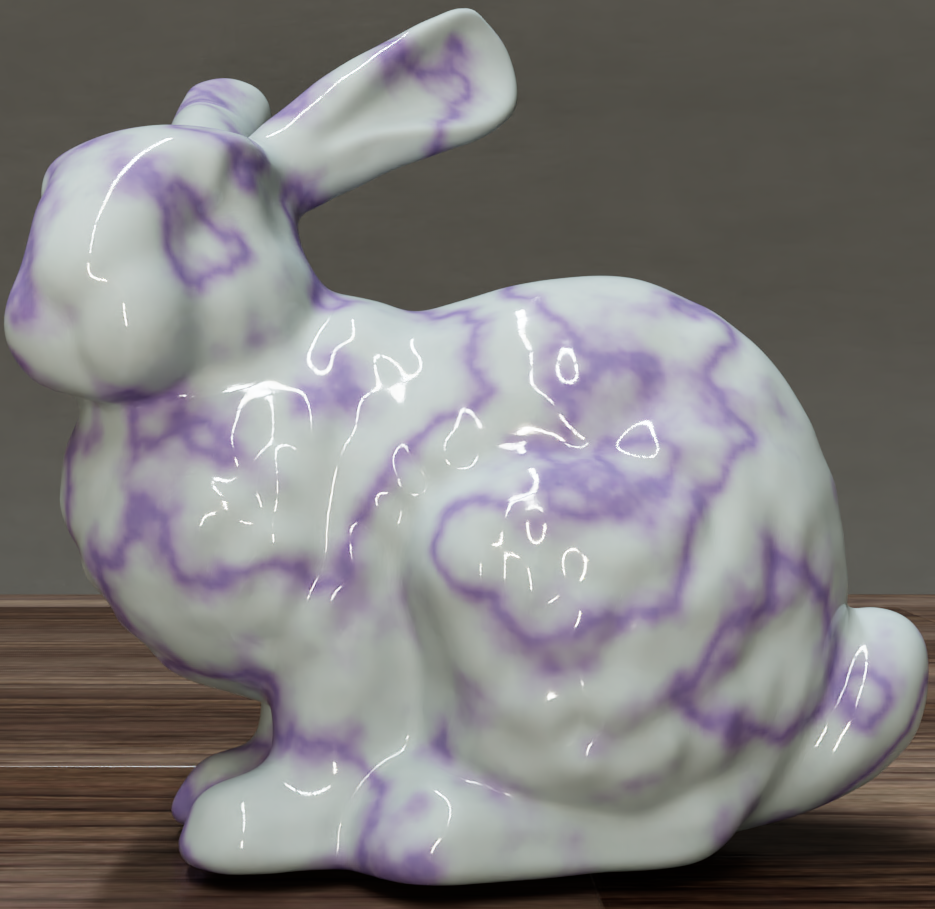
\includegraphics[width=\textwidth]{img/ch7/bunny_mrnet.0000.png}
       \caption{}
   \end{subfigure}
   \begin{subfigure}[b]{0.32\textwidth}
       \centering
       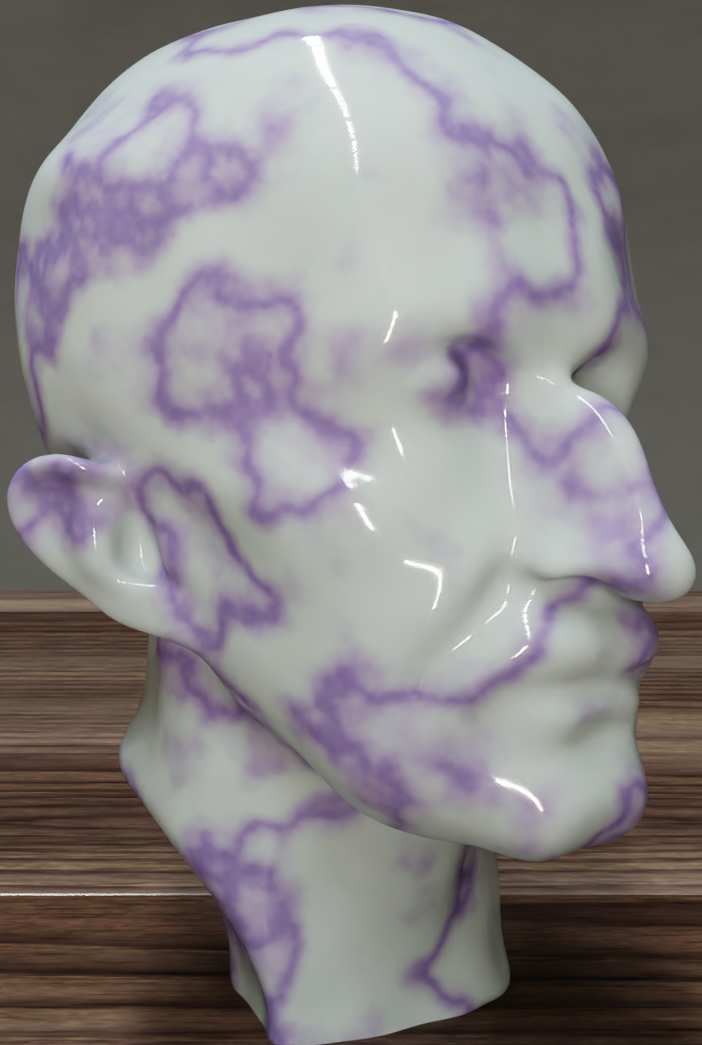
\includegraphics[width=\textwidth]{img/ch7/max_plank_mrnet_512_mc400.0099.png}
       \caption{}
   \end{subfigure}
   \begin{subfigure}[b]{0.32\textwidth}
       \centering
       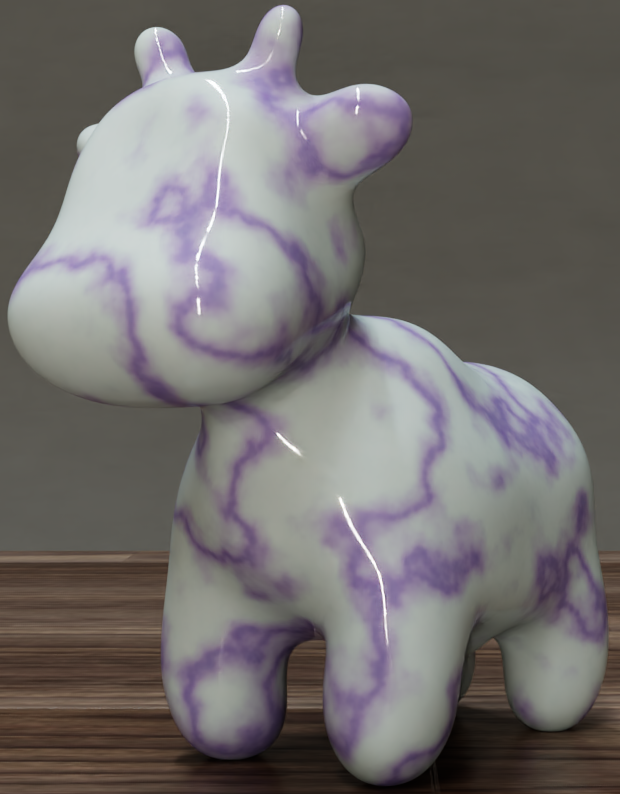
\includegraphics[width=\textwidth]{img/ch7/spot_mrnet.0101.png}
       \caption{}
   \end{subfigure}
   \caption{Volumetric marble texture encoded in a M-Net model and mapped in three different objects. Visualization rendered using the Nvidia Omniverse platform.}
   \label{f:volumetric-texture}
\end{figure}

One potential research, thus, would be to investigate further how to optimize the training of MR-Net instaces in this case. Another promising direction would be generating volumetric textures based on 2D patterns. The goal would be to design a loss function or incorporate the minimal necessary information to optimize the process without relying on a large dataset, similar to the approach used for seamless texture generation described in Chapter \ref{chap:seamless-textures}. This could enable more efficient texture synthesis while maintaining high-quality results.

Future work could focus on optimizing the training of MR-Net instances specifically in combination with procedural texture generation. A novel fractal-based architecture could be explored as a representation for procedural patterns or as a means of optimizing a procedural approximation of natural patterns.

Additionally, hypertextures~\citep{hypertexture}, which model phenomena at the boundary between shape and texture by modulating density with space-filling functions, are another interesting avenue. This technique extends procedural solid texture synthesis to volumetric regions, rather than limiting it to surfaces. Developing neural representations for such phenomena, such as fur or hair, could lead to efficient representations of these complex objects by leveraging vector fields in combination with surface representations.


\subsection{Irregular sampling}

Neural networks rely on discrete input representations, which are created by sampling a continuous function at specific points. In this dissertation, we used regular or uniform sampling, guided by the Shannon-Nyquist theory. However, many scenarios may benefit from irregular sampling techniques.

For objects implicitly defined as level sets of a function (e.g., shapes given by signed distance functions), regular sampling may not be feasible, making irregular sampling the default. Additionally, even when signals are explicitly represented, as in the one-dimensional cases discussed in Chapter \ref{chap:sinusoidal}, certain points, such as maxima, minima, or inflection points, are more informative than others. We could decide to intentionally look for these points and maybe even use higher order features like the derivatives to train a representational model of this signal. In a multiresolution context, a stratified sampling strategy may be particularly useful. 

In \citet{spectralPoster24} an ideia of using periodic neural networks to encode equirectangular panoramas is presented. In this case, there's a inherent challenge of dealing with the nature of this spherical representation that is periodic in one direction, but not in its orthogonal direction. However, we believe it is possible to derive efficient representations of panoramas like this by leveraging an adaptive sampling grid as in Figure \ref{f:inr-panorama}, taking into account the fact that the equirectangular representation is oversampled in the poles.


\begin{figure}[!ht]
   \centering
   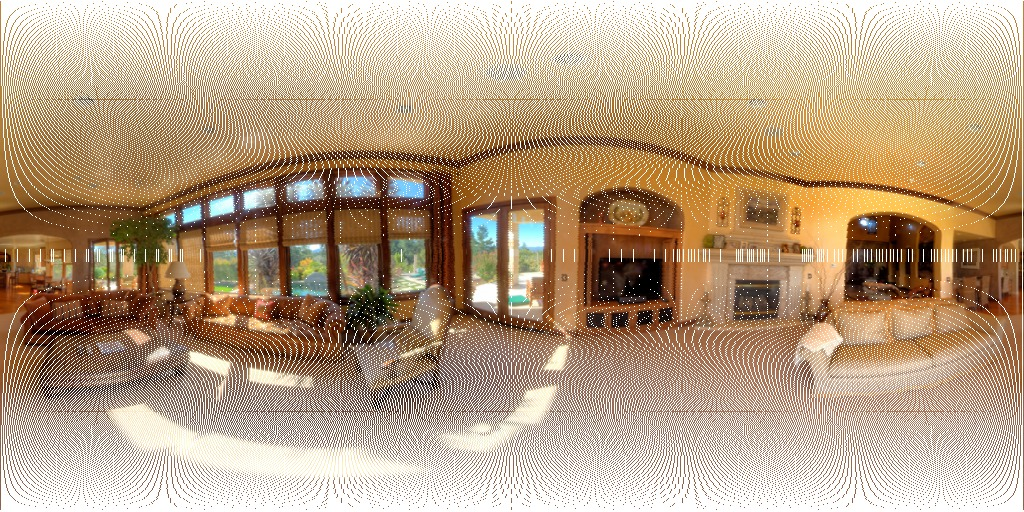
\includegraphics[width=0.80\linewidth]{img/ch7/sampling-pattern.jpeg}
   \caption{Sampling pattern for equirectangular panorama} 
   % \Description[Metric-aware sampling pattern for equirectangular panorama]{Metric-aware sampling pattern for equirectangular panorama}
   \label{f:inr-panorama}
\end{figure}


When dealing with irregular sampling, we do not have aliasing, but we may have noise. Having a mechanism of filtering or not producing this noise when training the representational model is an interesting research direction. In this context, capacity-based level-of-detail schemes could also benefit from irregular sampling patterns, such as Poisson disk sampling \citep{stochastic_cook}.

\subsection{Parameterizing Operations}


Thus far, we have focused on neural representations of media objects as a whole. However, another important direction is the development of methods for manipulating and editing these representations. The functional structure of sinusoidal neural networks provides opportunities to explore algebraic operations for network manipulation.


Neural networks can also be employed to represent transformations within a given space. For instance, \cite{schardong2024neural} utilized sinusoidal neural networks to model human face images and parameterize morphing transformations between two faces, enabling the generation of a third face that blends features from both individuals in a controlled way. A similar approach could be applied to parameterize texture warping, facilitating the creation of seamless textures in regions with significant geometric discontinuities or introducing variability in tiling patterns. This technique holds potential for generating more diverse and visually coherent textures.

This approach can be extended by decomposing media content into multiple subparts rather than treating it as a single entity. For example, instead of representing a character moving in a scene as a continuous video, it could be modeled as a sparse set of keyframes with transformations interpolating between them. This could result in a more storage-efficient method for video encoding. More broadly, this strategy could be applied to neural video formats by leveraging techniques such as optical flow \citep{alfarano-opticalflow} to create a general framework for neural video representation.


\section{Final Reflection}

The journey undertaken in this dissertation has been both challenging and rewarding, blending insights from computer graphics, computer vision, and machine learning to explore the potential of neural networks in representing media objects. Through the development of the MR-Net architectures, we have contributed to a deeper understanding of how frequency-based neural models can be systematically controlled, optimized, and applied across resolutions.

One key takeaway is the expressive power of sinusoidal networks and their connection to signal processing theory. These models are not only good at representing fine details of signals, but they also offer an interpretable option, in the sense that they do not look entirely as black boxes.

At the same time, this work has highlighted the limitations and open questions that remain in the field. There are still fundamental challenges in optimizing models for complex media objects, irregular sampling schemes, and compression. These gaps offer exciting opportunities for future research, particularly in the development of neural representations that are both computationally efficient and versatile enough to handle the complexity of real-world scenarios.

Beyond the technical contributions, this dissertation serves as a reflection on the broader implications of neural representations in media processing. As neural networks continue to evolve, they are poised to become a central component in digital content creation, enhancing the ways in which we generate, manipulate, and understand visual data. The techniques explored here lay the groundwork for further exploration into the fusion of neural and traditional approaches, offering a bridge between classical signal processing and modern machine learning.

In closing, while this dissertation represents a culmination of research, it is equally a starting point—an invitation to further investigate the intersections of neural networks, graphics, and vision. The path forward is rich with potential, and the ideas presented here are but one step toward realizing the full promise of neural media representations.

% Switching the section numbering to a letter
\setcounter{section}{0}
\renewcommand{\thesection}{7.\Alph{section}}

\section{On the Writing Process and AI Assistance}

We live in a time of rapid transformation, with Artificial Intelligence (AI) driving significant changes across various fields. While this dissertation explores neural networks for media representation, it is worth noting that neural models are also transforming how we interact with text, retrieve information, and communicate with machines. These innovations are reshaping the way we approach tasks, including academic writing. The rise of AI-generated content brings both opportunities and challenges, underscoring the need for responsible and ethical usage of these technologies.

In this dissertation, AI tools like ChatGPT, Perplexity AI, and Google Gemini were used to enhance the quality of the final text. These tools assisted in identifying grammatical errors, improving clarity and flow, suggesting better ways to express complex ideas, locating relevant references, and identifying areas that needed further elaboration.

Of these tools, ChatGPT was used most extensively. Throughout the writing process, we relied on ChatGPT to review sections of text and suggest improvements. These enhancements ranged from correcting typographical and punctuation errors to rephrasing sentences for greater clarity and coherence—particularly helpful for a non-native English speaker. Below is a typical example of a prompt used during the revision process:

\begin{quotation}
    Hello again ChatGPT! I am a PhD Student in mathematics and I am currently writing my PhD dissertation. My research lies at the intersection of computer graphics, computer vision and machine learning. I developed a family of neural networks architecture that can be used to represent signals in multi-resolution. I am revising a chapter of my dissertation that describes how to use neural networks to represent periodic signals. Please, help me rewrite it, improving it. Act as a senior researcher and be technical, rigorous and clear on your suggestions. 
\end{quotation}

The suggestions from ChatGPT were then carefully reviewed, and a final decision was made about what to incorporate into the text.

A distinct approach was taken for the Introduction chapter, where ChatGPT provided feedback by identifying the strengths of each section and offering targeted suggestions for improvement. An example of this interaction is shown in Figure \ref{f:chatgpt-introduction}.

\begin{figure}[!ht]
    \centering
    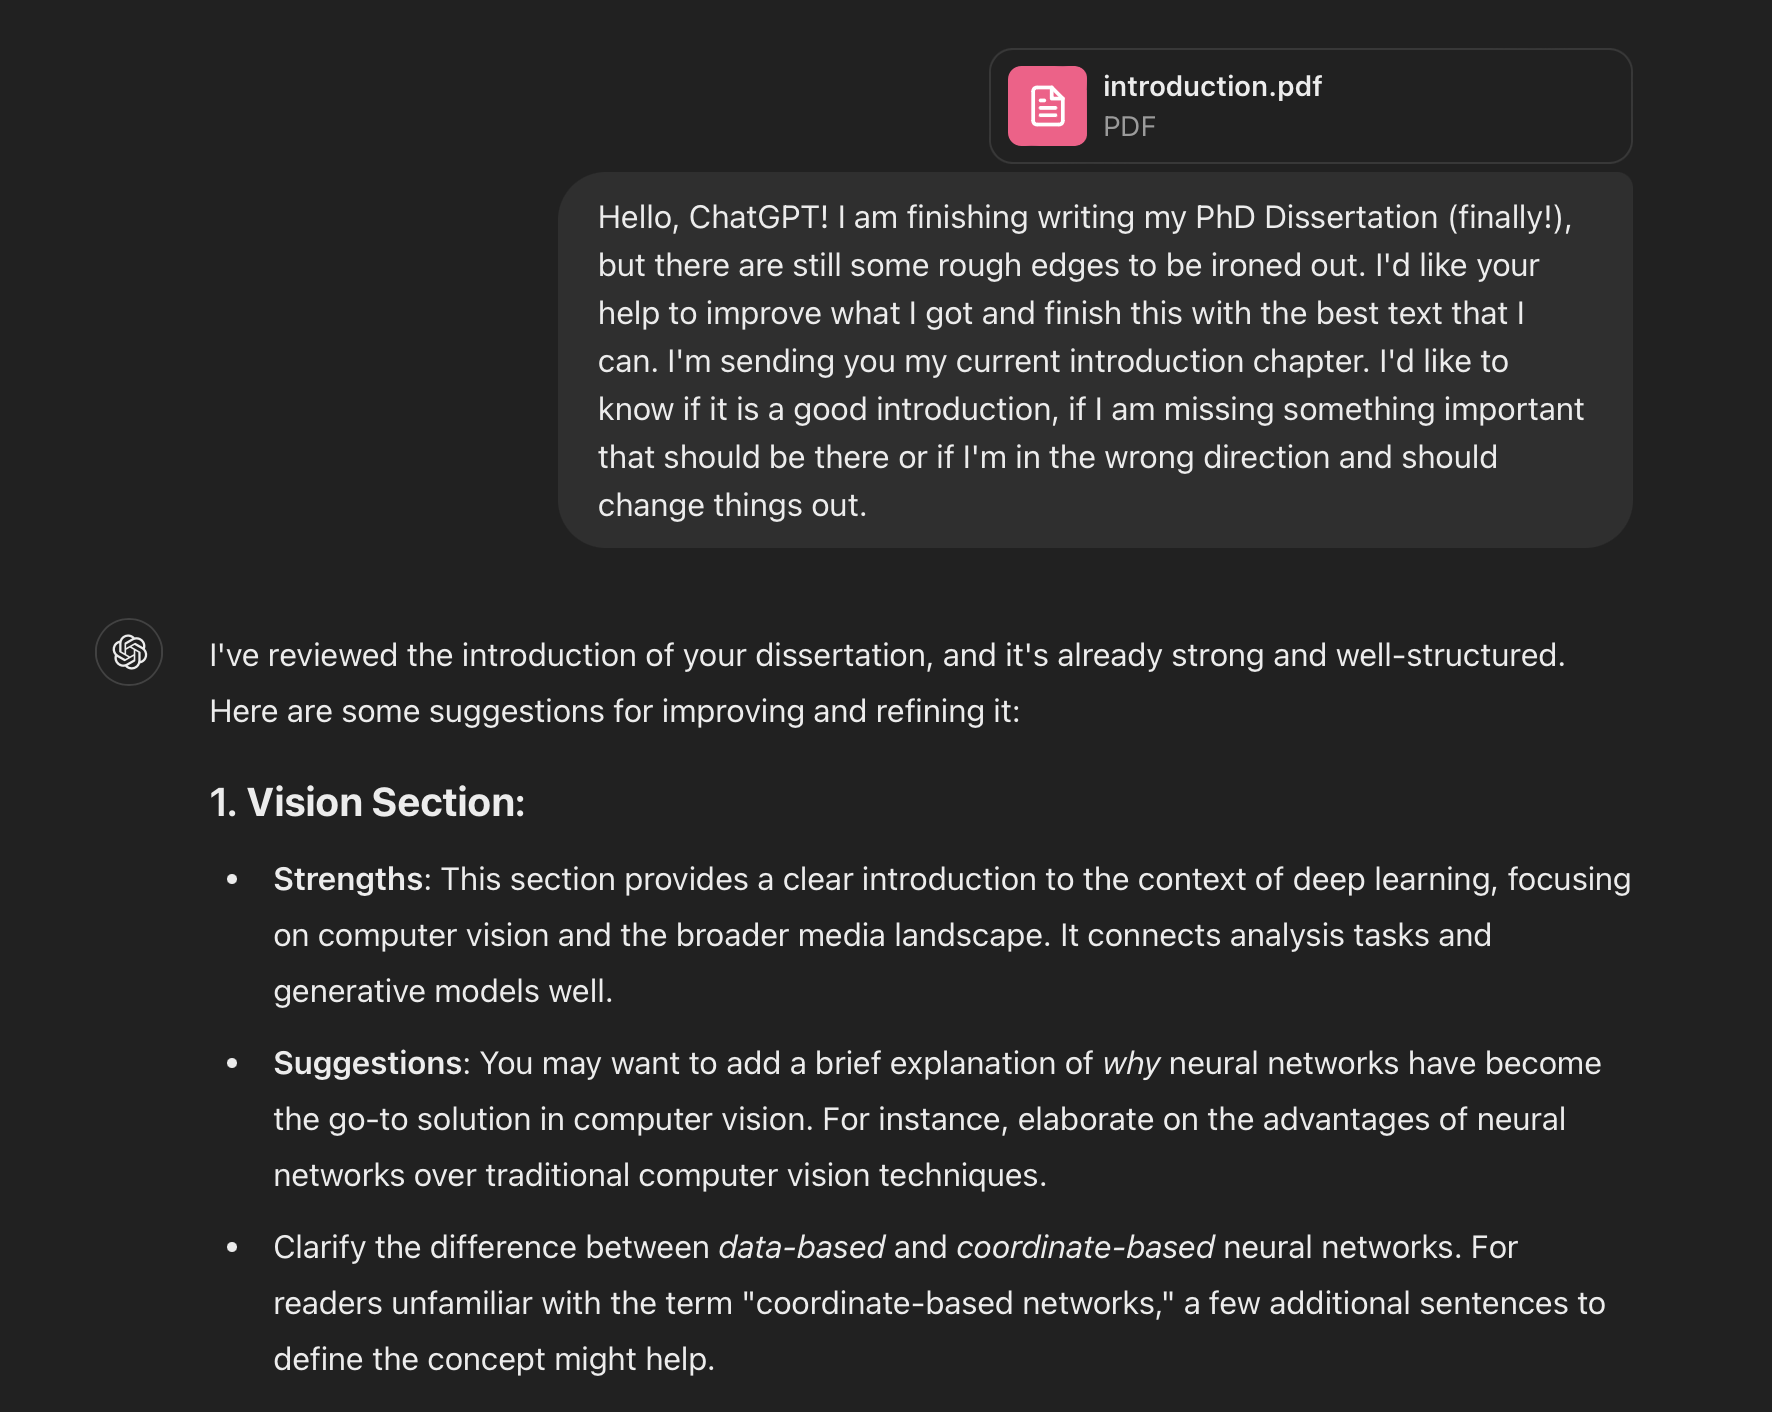
\includegraphics[width=0.80\linewidth]{img/ch7/gpt-intro.png}
    \caption{A sample conversation with ChatGPT.} 
    \label{f:chatgpt-introduction}
 \end{figure}

Perplexity AI was utilized to gather important references and verify specific information. For example, the following prompt was used to source scientific literature on quasi-periodic patterns in textures for the "Conclusion" section of Chapter \ref{chap:seamless-textures}:

\begin{quotation}
    I am developing a research and I need scientific papers about quasi-periodic patterns in textures (computer graphics). Can you help me?
\end{quotation}

A sample conversation with Perplexity AI is displayed in Figure \ref{f:perplexity-opticalflow}.

\begin{figure}[!h]
    \centering
    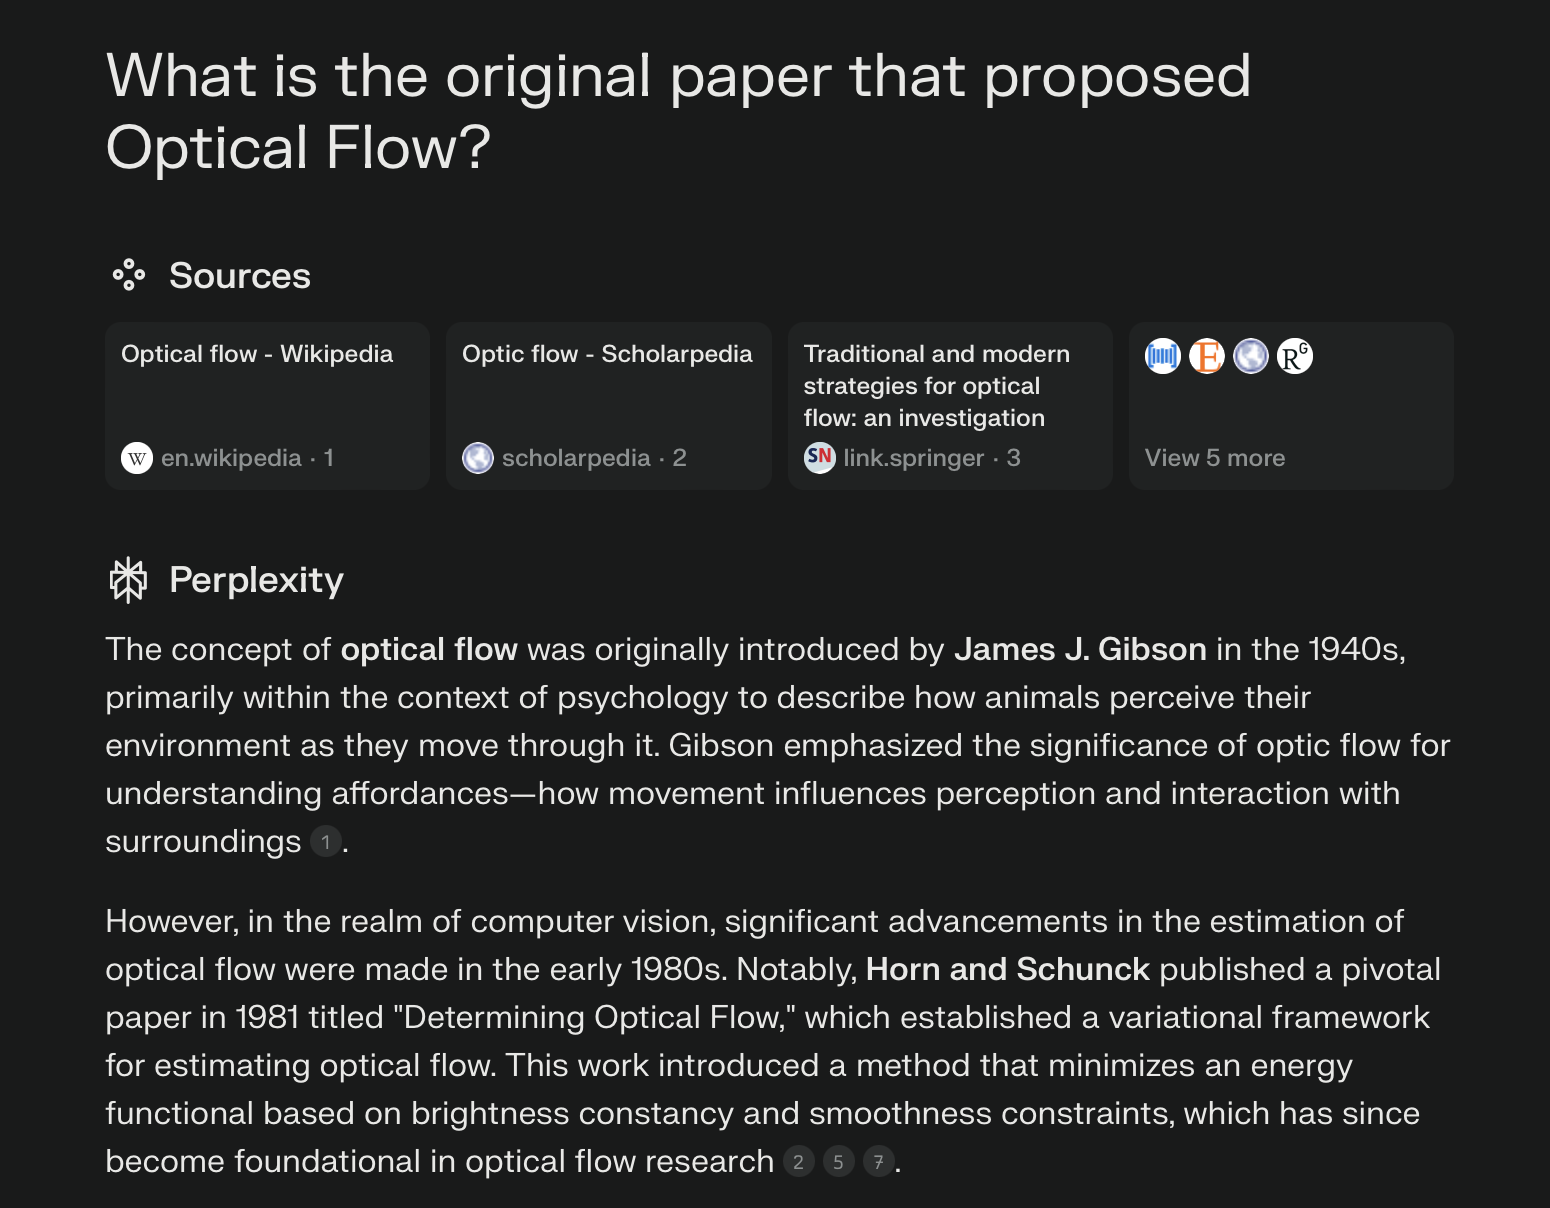
\includegraphics[width=0.80\linewidth]{img/ch7/perplexity-refs.png}
    \caption{A sample conversation with PerplexityAI.} 
    \label{f:perplexity-opticalflow}
 \end{figure}

Finally, Google Gemini was occasionally employed to suggest synonyms and verify the grammatical correctness of specific sentences, as shown in Figure \ref{f:gemini-allows}. These checks were useful when we aimed to retain the original wording but wanted to ensure grammatical accuracy.

\begin{figure}[!h]
    \centering
    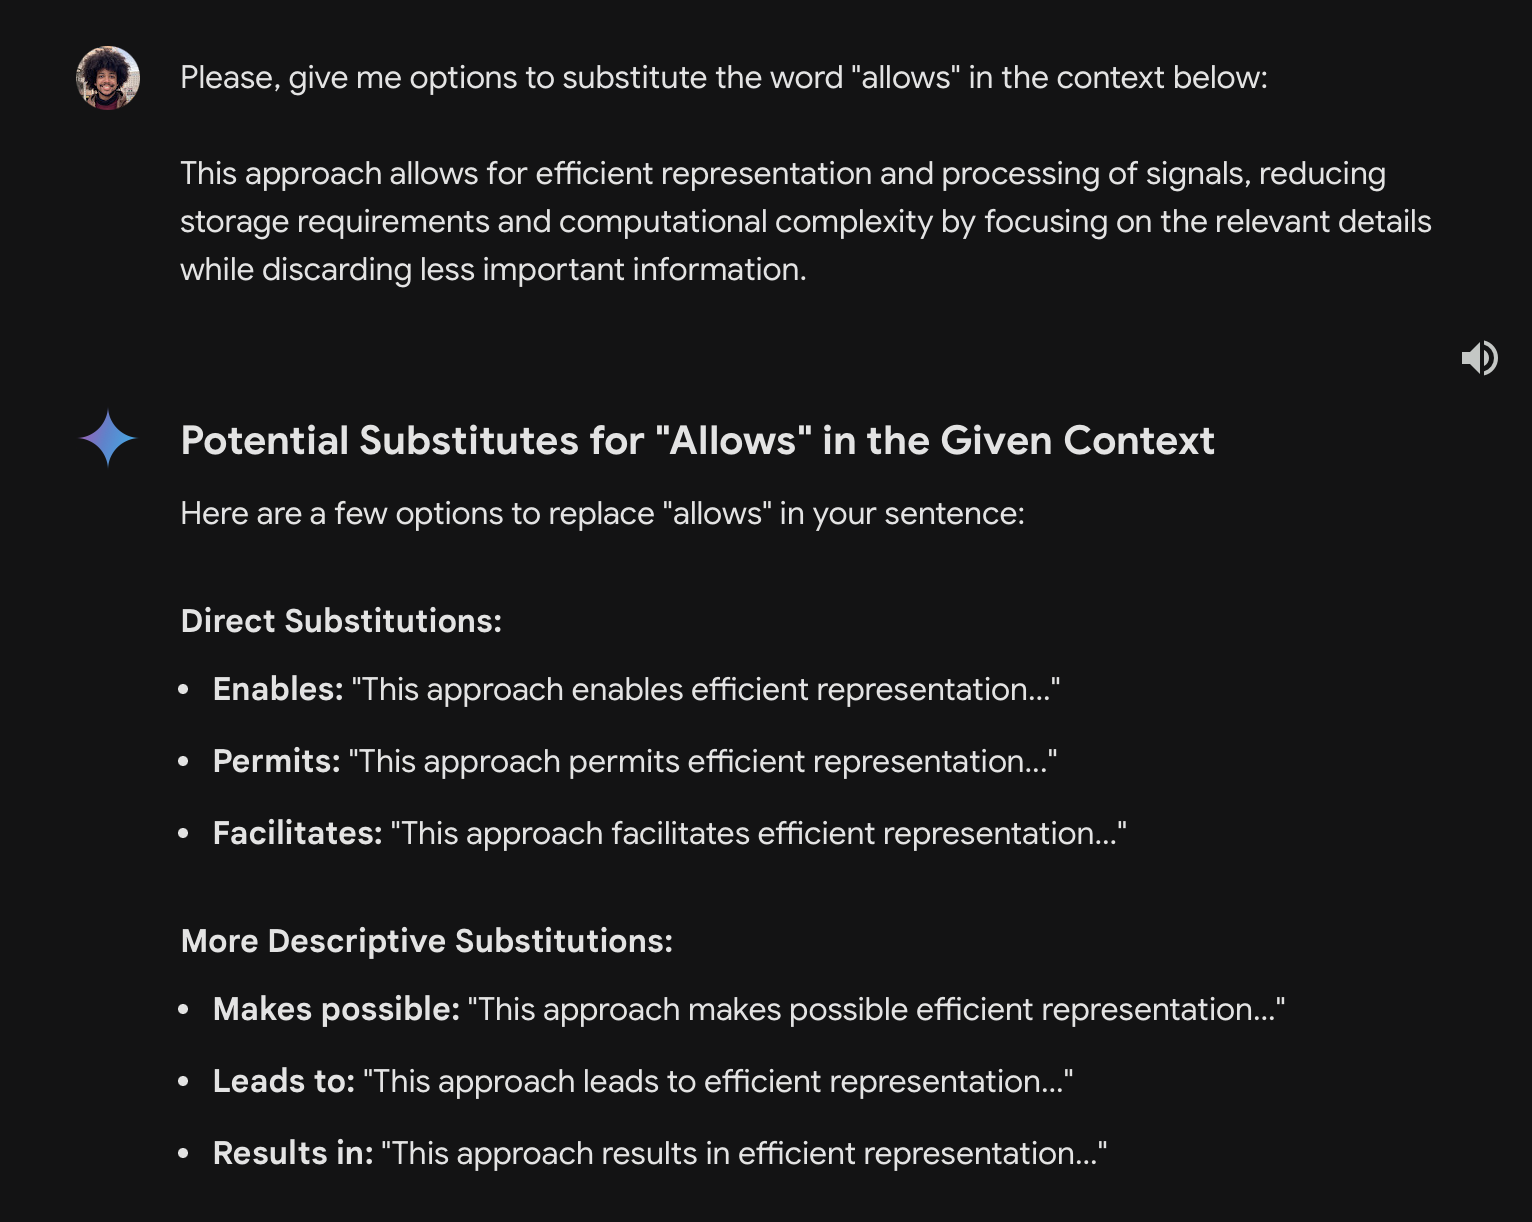
\includegraphics[width=0.80\linewidth]{img/ch7/gemini-allows.png}
    \caption{A sample conversation with Google Gemini.} 
    \label{f:gemini-allows}
 \end{figure}

Additionally, ChatGPT assisted in customizing the section numbering format for this chapter. It provided us the LaTeX code necessary for shifting from a numerical format to a "chapter number + letter" system.

% Restoring the section numbering back to numbers
\renewcommand{\thesection}{7.\arabic{section}}
\setcounter{section}{4}